% ============================================================================
% CAPITULO 4 - METODOLOGIA
% ============================================================================

\section{Metodologia}

% --- Slide: Arquitetura em Cascata ---
\begin{frame}{Arquitetura em Cascata}
  \vfill
  \begin{center}
    \resizebox{0.95\textwidth}{!}{% ============================================================================
% Diagrama da Arquitetura em Cascata - PGIE + 3 SGIEs (Simplificado)
% Para dissertação de mestrado PPGC/UFRGS
% Uso: % ============================================================================
% Diagrama da Arquitetura em Cascata - PGIE + 3 SGIEs (Simplificado)
% Para dissertação de mestrado PPGC/UFRGS
% Uso: % ============================================================================
% Diagrama da Arquitetura em Cascata - PGIE + 3 SGIEs (Simplificado)
% Para dissertação de mestrado PPGC/UFRGS
% Uso: \input{figuras/diagrama_cascata.tex}
% ============================================================================

\begin{tikzpicture}[
    scale=0.9, transform shape,
    % Estilos dos nós
    input/.style={
        rectangle,
        rounded corners=3pt,
        draw=black!60,
        fill=gray!15,
        minimum width=2.2cm,
        minimum height=1.0cm,
        align=center,
        font=\small\bfseries
    },
    pgie/.style={
        rectangle,
        rounded corners=4pt,
        draw=blue!60!black,
        fill=blue!20,
        minimum width=3.5cm,
        minimum height=1.2cm,
        align=center,
        font=\small\bfseries,
        line width=1pt
    },
    pgie_classes/.style={
        rectangle,
        rounded corners=3pt,
        draw=blue!40!black,
        fill=blue!8,
        minimum width=3.2cm,
        align=left,
        font=\scriptsize,
        inner sep=4pt
    },
    sgie/.style={
        rectangle,
        rounded corners=4pt,
        draw=teal!60!black,
        fill=teal!15,
        minimum width=3.0cm,
        minimum height=1.0cm,
        align=center,
        font=\small\bfseries,
        line width=0.8pt
    },
    sgie_classes/.style={
        rectangle,
        rounded corners=3pt,
        draw=teal!40!black,
        fill=teal!6,
        minimum width=2.8cm,
        align=left,
        font=\scriptsize,
        inner sep=4pt
    },
    output/.style={
        rectangle,
        rounded corners=3pt,
        draw=green!50!black,
        fill=green!12,
        minimum width=2.2cm,
        minimum height=1.0cm,
        align=center,
        font=\small\bfseries,
        line width=0.8pt
    },
    arrow/.style={->, >=stealth, thick, draw=black!50},
    arrow_pgie/.style={->, >=stealth, thick, draw=blue!50!black},
    arrow_sgie/.style={->, >=stealth, thick, draw=teal!50!black},
    label_arrow/.style={font=\scriptsize, fill=white, inner sep=1pt}
]

% ============================================================================
% Entrada
% ============================================================================
\node[input] (input) at (0, 0) {Frame de\\Vídeo};

% ============================================================================
% PGIE
% ============================================================================
\node[pgie] (pgie) at (3.8, 0) {PGIE\\(Detector Primário)};

\node[pgie_classes, anchor=north] (pgie_classes) at (3.8, -0.9) {
    \textbf{5 Classes:}\\
    Pessoa | Veículo | Capacete\\
    Colete | Ferramenta
};

% ============================================================================
% SGIEs
% ============================================================================
\node[sgie] (sgie_epi) at (8.5, 2.0) {SGIE-EPI};
\node[sgie_classes, anchor=north] (sgie_epi_classes) at (8.5, 1.4) {
    14 classes: EPIs,\\
    Quedas, Escadas...
};

\node[sgie] (sgie_maq) at (8.5, -0.3) {SGIE-Maquinário};
\node[sgie_classes, anchor=north] (sgie_maq_classes) at (8.5, -0.9) {
    Escavadeira, Guindaste\\
    Caminhão, Empilhadeira
};

\node[sgie] (sgie_fer) at (8.5, -2.6) {SGIE-Ferramentas};
\node[sgie_classes, anchor=north] (sgie_fer_classes) at (8.5, -3.2) {
    Escada, Cone\\
    Andaime, Carrinho
};

% ============================================================================
% Saída
% ============================================================================
\node[output] (output) at (12.5, -0.3) {Frame\\Anotado};

% ============================================================================
% Setas
% ============================================================================
\draw[arrow] (input.east) -- (pgie.west);

\draw[arrow_pgie] (pgie.east) -- ++(0.5,0) |- (sgie_epi.west) node[label_arrow, pos=0.25, above=2pt] {\scriptsize Person};
\draw[arrow_pgie] (pgie.east) -- ++(0.5,0) |- (sgie_maq.west) node[label_arrow, pos=0.25, above=2pt] {\scriptsize Vehicle};
\draw[arrow_pgie] (pgie.east) -- ++(0.5,0) |- (sgie_fer.west) node[label_arrow, pos=0.25, below=2pt] {\scriptsize Tool};

\draw[arrow_sgie] (sgie_epi.east) -- ++(0.4,0) |- (output.north west);
\draw[arrow_sgie] (sgie_maq.east) -- (output.west);
\draw[arrow_sgie] (sgie_fer.east) -- ++(0.4,0) |- (output.south west);

% ============================================================================
% Título
% ============================================================================
\node[font=\normalsize\bfseries, text=labelcolor] at (6.2, 3.5) {Arquitetura de Inferência em Cascata};

% Separador
\draw[dashed, gray!40, line width=0.4pt] (6.0, 3.2) -- (6.0, -4.2);

% Labels das seções
\node[font=\scriptsize, gray] at (1.9, -2.5) {Detector Primário};
\node[font=\scriptsize, gray] at (10.5, -4.6) {Detectores Secundários};

\end{tikzpicture}

% ============================================================================

\begin{tikzpicture}[
    scale=0.9, transform shape,
    % Estilos dos nós
    input/.style={
        rectangle,
        rounded corners=3pt,
        draw=black!60,
        fill=gray!15,
        minimum width=2.2cm,
        minimum height=1.0cm,
        align=center,
        font=\small\bfseries
    },
    pgie/.style={
        rectangle,
        rounded corners=4pt,
        draw=blue!60!black,
        fill=blue!20,
        minimum width=3.5cm,
        minimum height=1.2cm,
        align=center,
        font=\small\bfseries,
        line width=1pt
    },
    pgie_classes/.style={
        rectangle,
        rounded corners=3pt,
        draw=blue!40!black,
        fill=blue!8,
        minimum width=3.2cm,
        align=left,
        font=\scriptsize,
        inner sep=4pt
    },
    sgie/.style={
        rectangle,
        rounded corners=4pt,
        draw=teal!60!black,
        fill=teal!15,
        minimum width=3.0cm,
        minimum height=1.0cm,
        align=center,
        font=\small\bfseries,
        line width=0.8pt
    },
    sgie_classes/.style={
        rectangle,
        rounded corners=3pt,
        draw=teal!40!black,
        fill=teal!6,
        minimum width=2.8cm,
        align=left,
        font=\scriptsize,
        inner sep=4pt
    },
    output/.style={
        rectangle,
        rounded corners=3pt,
        draw=green!50!black,
        fill=green!12,
        minimum width=2.2cm,
        minimum height=1.0cm,
        align=center,
        font=\small\bfseries,
        line width=0.8pt
    },
    arrow/.style={->, >=stealth, thick, draw=black!50},
    arrow_pgie/.style={->, >=stealth, thick, draw=blue!50!black},
    arrow_sgie/.style={->, >=stealth, thick, draw=teal!50!black},
    label_arrow/.style={font=\scriptsize, fill=white, inner sep=1pt}
]

% ============================================================================
% Entrada
% ============================================================================
\node[input] (input) at (0, 0) {Frame de\\Vídeo};

% ============================================================================
% PGIE
% ============================================================================
\node[pgie] (pgie) at (3.8, 0) {PGIE\\(Detector Primário)};

\node[pgie_classes, anchor=north] (pgie_classes) at (3.8, -0.9) {
    \textbf{5 Classes:}\\
    Pessoa | Veículo | Capacete\\
    Colete | Ferramenta
};

% ============================================================================
% SGIEs
% ============================================================================
\node[sgie] (sgie_epi) at (8.5, 2.0) {SGIE-EPI};
\node[sgie_classes, anchor=north] (sgie_epi_classes) at (8.5, 1.4) {
    14 classes: EPIs,\\
    Quedas, Escadas...
};

\node[sgie] (sgie_maq) at (8.5, -0.3) {SGIE-Maquinário};
\node[sgie_classes, anchor=north] (sgie_maq_classes) at (8.5, -0.9) {
    Escavadeira, Guindaste\\
    Caminhão, Empilhadeira
};

\node[sgie] (sgie_fer) at (8.5, -2.6) {SGIE-Ferramentas};
\node[sgie_classes, anchor=north] (sgie_fer_classes) at (8.5, -3.2) {
    Escada, Cone\\
    Andaime, Carrinho
};

% ============================================================================
% Saída
% ============================================================================
\node[output] (output) at (12.5, -0.3) {Frame\\Anotado};

% ============================================================================
% Setas
% ============================================================================
\draw[arrow] (input.east) -- (pgie.west);

\draw[arrow_pgie] (pgie.east) -- ++(0.5,0) |- (sgie_epi.west) node[label_arrow, pos=0.25, above=2pt] {\scriptsize Person};
\draw[arrow_pgie] (pgie.east) -- ++(0.5,0) |- (sgie_maq.west) node[label_arrow, pos=0.25, above=2pt] {\scriptsize Vehicle};
\draw[arrow_pgie] (pgie.east) -- ++(0.5,0) |- (sgie_fer.west) node[label_arrow, pos=0.25, below=2pt] {\scriptsize Tool};

\draw[arrow_sgie] (sgie_epi.east) -- ++(0.4,0) |- (output.north west);
\draw[arrow_sgie] (sgie_maq.east) -- (output.west);
\draw[arrow_sgie] (sgie_fer.east) -- ++(0.4,0) |- (output.south west);

% ============================================================================
% Título
% ============================================================================
\node[font=\normalsize\bfseries, text=labelcolor] at (6.2, 3.5) {Arquitetura de Inferência em Cascata};

% Separador
\draw[dashed, gray!40, line width=0.4pt] (6.0, 3.2) -- (6.0, -4.2);

% Labels das seções
\node[font=\scriptsize, gray] at (1.9, -2.5) {Detector Primário};
\node[font=\scriptsize, gray] at (10.5, -4.6) {Detectores Secundários};

\end{tikzpicture}

% ============================================================================

\begin{tikzpicture}[
    scale=0.9, transform shape,
    % Estilos dos nós
    input/.style={
        rectangle,
        rounded corners=3pt,
        draw=black!60,
        fill=gray!15,
        minimum width=2.2cm,
        minimum height=1.0cm,
        align=center,
        font=\small\bfseries
    },
    pgie/.style={
        rectangle,
        rounded corners=4pt,
        draw=blue!60!black,
        fill=blue!20,
        minimum width=3.5cm,
        minimum height=1.2cm,
        align=center,
        font=\small\bfseries,
        line width=1pt
    },
    pgie_classes/.style={
        rectangle,
        rounded corners=3pt,
        draw=blue!40!black,
        fill=blue!8,
        minimum width=3.2cm,
        align=left,
        font=\scriptsize,
        inner sep=4pt
    },
    sgie/.style={
        rectangle,
        rounded corners=4pt,
        draw=teal!60!black,
        fill=teal!15,
        minimum width=3.0cm,
        minimum height=1.0cm,
        align=center,
        font=\small\bfseries,
        line width=0.8pt
    },
    sgie_classes/.style={
        rectangle,
        rounded corners=3pt,
        draw=teal!40!black,
        fill=teal!6,
        minimum width=2.8cm,
        align=left,
        font=\scriptsize,
        inner sep=4pt
    },
    output/.style={
        rectangle,
        rounded corners=3pt,
        draw=green!50!black,
        fill=green!12,
        minimum width=2.2cm,
        minimum height=1.0cm,
        align=center,
        font=\small\bfseries,
        line width=0.8pt
    },
    arrow/.style={->, >=stealth, thick, draw=black!50},
    arrow_pgie/.style={->, >=stealth, thick, draw=blue!50!black},
    arrow_sgie/.style={->, >=stealth, thick, draw=teal!50!black},
    label_arrow/.style={font=\scriptsize, fill=white, inner sep=1pt}
]

% ============================================================================
% Entrada
% ============================================================================
\node[input] (input) at (0, 0) {Frame de\\Vídeo};

% ============================================================================
% PGIE
% ============================================================================
\node[pgie] (pgie) at (3.8, 0) {PGIE\\(Detector Primário)};

\node[pgie_classes, anchor=north] (pgie_classes) at (3.8, -0.9) {
    \textbf{5 Classes:}\\
    Pessoa | Veículo | Capacete\\
    Colete | Ferramenta
};

% ============================================================================
% SGIEs
% ============================================================================
\node[sgie] (sgie_epi) at (8.5, 2.0) {SGIE-EPI};
\node[sgie_classes, anchor=north] (sgie_epi_classes) at (8.5, 1.4) {
    14 classes: EPIs,\\
    Quedas, Escadas...
};

\node[sgie] (sgie_maq) at (8.5, -0.3) {SGIE-Maquinário};
\node[sgie_classes, anchor=north] (sgie_maq_classes) at (8.5, -0.9) {
    Escavadeira, Guindaste\\
    Caminhão, Empilhadeira
};

\node[sgie] (sgie_fer) at (8.5, -2.6) {SGIE-Ferramentas};
\node[sgie_classes, anchor=north] (sgie_fer_classes) at (8.5, -3.2) {
    Escada, Cone\\
    Andaime, Carrinho
};

% ============================================================================
% Saída
% ============================================================================
\node[output] (output) at (12.5, -0.3) {Frame\\Anotado};

% ============================================================================
% Setas
% ============================================================================
\draw[arrow] (input.east) -- (pgie.west);

\draw[arrow_pgie] (pgie.east) -- ++(0.5,0) |- (sgie_epi.west) node[label_arrow, pos=0.25, above=2pt] {\scriptsize Person};
\draw[arrow_pgie] (pgie.east) -- ++(0.5,0) |- (sgie_maq.west) node[label_arrow, pos=0.25, above=2pt] {\scriptsize Vehicle};
\draw[arrow_pgie] (pgie.east) -- ++(0.5,0) |- (sgie_fer.west) node[label_arrow, pos=0.25, below=2pt] {\scriptsize Tool};

\draw[arrow_sgie] (sgie_epi.east) -- ++(0.4,0) |- (output.north west);
\draw[arrow_sgie] (sgie_maq.east) -- (output.west);
\draw[arrow_sgie] (sgie_fer.east) -- ++(0.4,0) |- (output.south west);

% ============================================================================
% Título
% ============================================================================
\node[font=\normalsize\bfseries, text=labelcolor] at (6.2, 3.5) {Arquitetura de Inferência em Cascata};

% Separador
\draw[dashed, gray!40, line width=0.4pt] (6.0, 3.2) -- (6.0, -4.2);

% Labels das seções
\node[font=\scriptsize, gray] at (1.9, -2.5) {Detector Primário};
\node[font=\scriptsize, gray] at (10.5, -4.6) {Detectores Secundários};

\end{tikzpicture}
}
  \end{center}

  \vspace{2mm}

  % Annotation bar
  \begin{center}
    \small
    \begin{tikzpicture}
      \node[fill=blue!10, rounded corners=3pt, inner sep=4pt, font=\footnotesize]
        (flow) {%
          \textbf{Fluxo:}\;
          Frame $\;\xrightarrow{\text{PGIE}}\;$
          5 classes $\;\xrightarrow{\text{ROI crop}}\;$
          3 SGIEs especializados $\;\rightarrow\;$
          \textbf{46 categorias}
        };
    \end{tikzpicture}
  \end{center}

  \vspace{1mm}

  \begin{block}{}
    \centering\small
    \textbf{Vantagem:} cada SGIE opera apenas sobre a ROI relevante
    --- menor carga computacional e maior precisao por dominio.
  \end{block}
  \vfill
\end{frame}

% --- Slide: Classes do Sistema ---
\begin{frame}{Classes do Sistema}
  \vfill
  \begin{columns}[c]
    \begin{column}{0.62\textwidth}
      \centering
      \small
      \renewcommand{\arraystretch}{1.25}
      \begin{tabular}{@{}lclc@{}}
        \toprule
        \textbf{Modelo} & \textbf{Cls.} & \textbf{Entrada} & \textbf{Saida} \\
        \midrule
        \rowcolor{inputcolor!12}
        PGIE & 5 & Frame completo & Person, Vehicle, Hardhat, Vest, Tool \\
        \midrule
        \rowcolor{headcolor!12}
        SGIE-EPI & 14 & ROI \textit{Person} & \scriptsize Capacete, colete, oculos, luva, bota\ldots \\
        \rowcolor{neckcolor!12}
        SGIE-Maquinario & 9 & ROI \textit{Vehicle} & \scriptsize Escavadeira, guindaste, betoneira\ldots \\
        \rowcolor{outputcolor!12}
        SGIE-Ferramentas & 23 & ROI \textit{Tool} & \scriptsize Serra, furadeira, martelo, andaime\ldots \\
        \midrule
        \rowcolor{labelcolor!8}
        \textbf{Total} & \textbf{46} & & \textbf{\textit{categorias unicas}} \\
        \bottomrule
      \end{tabular}
    \end{column}
    \begin{column}{0.35\textwidth}
      \centering
      \begin{tikzpicture}[
        every node/.style={font=\scriptsize, align=center, minimum width=22mm,
                           minimum height=7mm, rounded corners=2pt},
        arr/.style={-{Latex[length=1.5mm]}, thick}
      ]
        \node[fill=inputcolor!20, draw=inputcolor!60] (pgie) at (0,0) {\textbf{PGIE}\\5 classes};
        \node[fill=headcolor!15, draw=headcolor!60] (s1) at (-0.8,-1.4) {\textbf{SGIE-EPI}\\14 cls};
        \node[fill=neckcolor!15, draw=neckcolor!60] (s2) at (0,-2.5) {\textbf{SGIE-Maq}\\9 cls};
        \node[fill=outputcolor!15, draw=outputcolor!60] (s3) at (0.8,-3.6) {\textbf{SGIE-Fer}\\23 cls};

        \draw[arr, headcolor!70] (pgie.south west) -- node[left, font=\tiny] {Person} (s1.north);
        \draw[arr, neckcolor!70] (pgie.south) -- node[right, font=\tiny] {Vehicle} (s2.north);
        \draw[arr, outputcolor!70] (pgie.south east) -- node[right, font=\tiny] {Tool} (s3.north);
      \end{tikzpicture}
    \end{column}
  \end{columns}
  \vfill
\end{frame}

% --- Slide: Datasets ---
\begin{frame}{Datasets}
  \vfill
  \centering
  \small
  \renewcommand{\arraystretch}{1.2}
  \begin{tabular}{@{}llcll@{}}
    \toprule
    \textbf{Modelo} & \textbf{Dataset} & \textbf{Classes} & \textbf{Foco} & \textbf{Tipo} \\
    \midrule
    \rowcolor{inputcolor!8}
    \multirow{3}{*}{PGIE} & SODA & 20 & Canteiros reais & Publico \\
    \rowcolor{inputcolor!8}
                           & MOCS & -- & Maquinas e equipamentos & Publico \\
    \rowcolor{inputcolor!8}
                           & Roboflow Construction & -- & Complementos & Publico \\
    \midrule
    \rowcolor{headcolor!8}
    \multirow{3}{*}{SGIE-EPI} & SHWD & 2 & Capacetes (${\sim}7.500$ img) & Publico \\
    \rowcolor{headcolor!8}
                               & GDUT-HWD & 2 & Capacetes verificados & Publico \\
    \rowcolor{headcolor!8}
                               & PPE Detection & 6+ & Multiplos EPIs & Roboflow \\
    \midrule
    \rowcolor{neckcolor!8}
    SGIE-Maq. & Construction Vehicles + Heavy Equip. & 9 & Maquinario pesado & Publico \\
    \midrule
    \rowcolor{outputcolor!8}
    SGIE-Fer. & Construction Tools + Safety Equip. & 23 & Ferramentas e materiais & Publico \\
    \bottomrule
  \end{tabular}

  \vspace{4mm}

  \begin{columns}[c]
    \begin{column}{0.48\textwidth}
      \begin{block}{Formato}
        \centering\footnotesize
        Todas as anotacoes convertidas para \textbf{YOLO format}\\
        (\texttt{class x\_center y\_center w h})
      \end{block}
    \end{column}
    \begin{column}{0.48\textwidth}
      \begin{alertblock}{Split (todos os modelos)}
        \centering\footnotesize
        \textbf{70\% / 20\% / 10\%}\\
        treino / validacao / teste
      \end{alertblock}
    \end{column}
  \end{columns}
  \vfill
\end{frame}

% --- Slide: Curadoria dos Datasets ---
\begin{frame}{Curadoria dos Datasets}
  \vfill
  \begin{center}
    \resizebox{0.92\textwidth}{!}{%
    \begin{tikzpicture}[
      step/.style={rectangle, rounded corners=4pt, draw=#1!60!black,
                   fill=#1!15, minimum width=28mm, minimum height=12mm,
                   align=center, font=\footnotesize\bfseries, line width=0.8pt},
      arr/.style={-{Latex[length=2mm]}, thick, draw=arrowcolor},
      note/.style={font=\tiny, text=sublabelcolor, align=center}
    ]
      \node[step=inputcolor] (s1) at (0,0) {Coleta de\\Datasets};
      \node[step=neckcolor]  (s2) at (3.5,0) {Remocao de\\Duplicatas};
      \node[step=headcolor]  (s3) at (7,0) {Padronizacao\\de Classes};
      \node[step=outputcolor](s4) at (10.5,0) {Balanceamento\\por Classe};
      \node[step=detectioncolor](s5) at (14,0) {Split\\70/20/10};

      \draw[arr] (s1) -- (s2);
      \draw[arr] (s2) -- (s3);
      \draw[arr] (s3) -- (s4);
      \draw[arr] (s4) -- (s5);

      \node[note, below=4mm of s1] {SODA, MOCS,\\SHWD, Roboflow};
      \node[note, below=4mm of s2] {\textit{Hashing}\\perceptual};
      \node[note, below=4mm of s3] {Mapeamento\\entre datasets};
      \node[note, below=4mm of s4] {Sub/sobre-\\amostragem};
      \node[note, below=4mm of s5] {Treino/val./teste\\estratificado};
    \end{tikzpicture}
    }
  \end{center}

  \vspace{4mm}

  \begin{columns}[c]
    \begin{column}{0.48\textwidth}
      \begin{block}{Verificacao Manual}
        \begin{itemize}\footnotesize
          \item Revisao de anotacoes incorretas
          \item Correcao de \textit{bounding boxes}
          \item Remocao de imagens corrompidas
        \end{itemize}
      \end{block}
    \end{column}
    \begin{column}{0.48\textwidth}
      \begin{block}{Padronizacao}
        \begin{itemize}\footnotesize
          \item Unificacao de \textit{labels} entre fontes
          \item Conversao para formato YOLO
          \item Resolucao de conflitos de classe
        \end{itemize}
      \end{block}
    \end{column}
  \end{columns}
  \vfill
\end{frame}

% --- Slide: Distribuicao PGIE ---
\begin{frame}{Distribuicao de Classes --- PGIE}
  \vfill
  \begin{columns}[c]
    \begin{column}{0.6\textwidth}
      \centering
      
\includegraphics[width=\textwidth]{labels_pgie.jpg}
    \end{column}
    \begin{column}{0.37\textwidth}
      \textbf{5 classes:}
      \vspace{2mm}
      \begin{itemize}\small
        \item Person, Vehicle, Hardhat,\\Safety Vest, Tool
        \vspace{2mm}
        \item Classe \textit{Person} predominante\\--- reflete cenarios reais
        \vspace{2mm}
        \item Desbalanceamento natural mitigado via \textit{data augmentation}
      \end{itemize}

      \vspace{3mm}

      \begin{block}{\footnotesize Distribuicao Espacial}
        \footnotesize
        Concentracao central com dispersao uniforme --- boa cobertura do campo visual.
      \end{block}
    \end{column}
  \end{columns}
  \vfill
\end{frame}

% --- Slide: Distribuicao SGIEs ---
\begin{frame}{Distribuicao de Classes --- SGIEs}
  \vfill
  \begin{columns}[c]
    \begin{column}{0.5\textwidth}
      \centering
      {\footnotesize\textbf{SGIE-Ferramentas} (23 classes)}\\[2mm]
      
\includegraphics[width=\textwidth]{labels_sgie_equipment.jpg}

      \vspace{1mm}
      {\tiny Desbalanceamento significativo entre categorias}
    \end{column}
    \begin{column}{0.5\textwidth}
      \centering
      {\footnotesize\textbf{SGIE-Maquinario} (9 classes)}\\[2mm]
      
\includegraphics[width=\textwidth]{labels_sgie_machinery.jpg}

      \vspace{1mm}
      {\tiny Distribuicao mais equilibrada entre as classes}
    \end{column}
  \end{columns}

  \vspace{3mm}

  \begin{block}{}
    \centering\footnotesize
    O SGIE-EPI (14 classes) utiliza datasets especializados (SHWD, GDUT-HWD, PPE Detection)
    com foco em presenca/ausencia de EPIs --- distribuicao controlada por par positivo/negativo.
  \end{block}
  \vfill
\end{frame}

% --- Slide: Data Augmentation ---
\begin{frame}{Data Augmentation}
  \vfill
  \begin{columns}[c]
    \begin{column}{0.57\textwidth}
      \centering
      
\includegraphics[width=\textwidth]{train_batch0.jpg}\\[1mm]
      {\tiny Amostra de batch de treinamento com augmentations aplicadas}
    \end{column}
    \begin{column}{0.40\textwidth}
      \textbf{Tecnicas e propositos:}
      \vspace{2mm}
      \begin{itemize}\small
        \item \textbf{Mosaic} (p=1.0)\\
          {\scriptsize Multi-escala, contexto variado}
        \vspace{2mm}
        \item \textbf{Flip horizontal} (p=0.5)\\
          {\scriptsize Invariancia a orientacao}
        \vspace{2mm}
        \item \textbf{Escala} (0.5x--1.5x)\\
          {\scriptsize Robustez a tamanhos variados}
        \vspace{2mm}
        \item \textbf{HSV} (h=0.015, s=0.7, v=0.4)\\
          {\scriptsize Invariancia a iluminacao}
        \vspace{2mm}
        \item \textbf{Translacao} (10\%)\\
          {\scriptsize Variacao de posicao}
      \end{itemize}
    \end{column}
  \end{columns}
  \vfill
\end{frame}

% --- Slide: Hiperparametros de Treinamento ---
\begin{frame}{Treinamento --- Hiperparametros}
  \vfill
  \begin{center}
    \small
    \renewcommand{\arraystretch}{1.25}
    \begin{tabular}{@{}lcc@{}}
      \toprule
      \textbf{Parametro} & \textbf{PGIE} & \textbf{SGIEs} \\
      \midrule
      \rowcolor{bgbox}
      Modelo base & YOLOv8m & YOLOv8s \\
      Resolucao & $640 \times 640$ & $320 \times 320$ \\
      \rowcolor{bgbox}
      Batch size & 16 & 32 \\
      Epocas maximas & 300 & 200 \\
      \rowcolor{bgbox}
      Otimizador & SGD & SGD \\
      LR inicial ($lr_0$) & 0,01 & 0,01 \\
      \rowcolor{bgbox}
      LR final ($lr_f$) & 0,01 & 0,01 \\
      Momentum & 0,937 & 0,937 \\
      \rowcolor{bgbox}
      Weight decay & 0,0005 & 0,0005 \\
      Warmup epochs & 3,0 & 3,0 \\
      \rowcolor{bgbox}
      Early stopping & 50 epocas & 30 epocas \\
      \bottomrule
    \end{tabular}
  \end{center}

  \vspace{3mm}

  \begin{columns}[c]
    \begin{column}{0.48\textwidth}
      \begin{block}{\footnotesize Funcao de Perda}
        \footnotesize
        $\mathcal{L} = \lambda_{box}\mathcal{L}_{box} + \lambda_{dfl}\mathcal{L}_{dfl} + \lambda_{cls}\mathcal{L}_{cls}$\\[1mm]
        {\scriptsize CIoU + Distribution Focal + BCE}
      \end{block}
    \end{column}
    \begin{column}{0.48\textwidth}
      \begin{block}{\footnotesize Ambiente}
        \footnotesize
        RTX 4070 (12\,GB), PyTorch 2.0\\
        Ultralytics YOLOv8 v8.0
      \end{block}
    \end{column}
  \end{columns}
  \vfill
\end{frame}

% --- Slide: Pipeline de Otimizacao ---
\begin{frame}{Pipeline de Otimizacao para Borda}
  \vfill
  \begin{center}
    \resizebox{0.95\textwidth}{!}{%
    \begin{tikzpicture}[node distance=16mm]
      \node[inputblock, minimum width=28mm, minimum height=14mm]
        (pt) {\textbf{PyTorch}\\(.pt)};
      \node[backboneblock, right=of pt, minimum width=28mm, minimum height=14mm]
        (onnx) {\textbf{ONNX}\\(.onnx)};
      \node[detectionblock, right=of onnx, minimum width=32mm, minimum height=14mm]
        (trt) {\textbf{TensorRT}\\FP16 (.engine)};
      \node[outputblock, right=of trt, minimum width=28mm, minimum height=14mm]
        (ds) {\textbf{DeepStream}\\Inferencia};

      \draw[arrow] (pt) -- node[above, font=\scriptsize\bfseries] {export} (onnx);
      \draw[arrow] (onnx) -- node[above, font=\scriptsize\bfseries] {otimizacao} (trt);
      \draw[arrow] (trt) -- node[above, font=\scriptsize\bfseries] {deploy} (ds);

      % Annotations below
      \node[below=5mm of pt, font=\tiny, align=center, text=sublabelcolor]
        {Treinamento\\GPU desktop};
      \node[below=5mm of onnx, font=\tiny, align=center, text=sublabelcolor]
        {Formato\\intermediario};
      \node[below=5mm of trt, font=\tiny, align=center, text=sublabelcolor]
        {Quantizacao FP16\\Fusao de camadas};
      \node[below=5mm of ds, font=\tiny, align=center, text=sublabelcolor]
        {Jetson AGX Xavier\\tempo real};
    \end{tikzpicture}
    }
  \end{center}

  \vspace{5mm}

  \begin{columns}[c]
    \begin{column}{0.48\textwidth}
      \begin{block}{\footnotesize Otimizacoes TensorRT}
        \begin{itemize}\scriptsize
          \item \textbf{Quantizacao FP16}: speedup ${\sim}$1.5--2x
          \item \textbf{Fusao de camadas}: Conv+BN+ReLU
          \item \textbf{Selecao de kernels}: otimizados p/ GPU alvo
        \end{itemize}
      \end{block}
    \end{column}
    \begin{column}{0.48\textwidth}
      \begin{block}{\footnotesize Conversao no Dispositivo}
        \begin{itemize}\scriptsize
          \item Compilado \textbf{diretamente no Jetson}
          \item Garante otimizacao especifica p/ hw
          \item Engine nao portavel entre GPUs
        \end{itemize}
      \end{block}
    \end{column}
  \end{columns}
  \vfill
\end{frame}
